\documentclass[11pt,a4paper]{article}

\usepackage[T1]{fontenc}
\usepackage[utf8]{inputenc}
\usepackage{lmodern}
\usepackage[english]{babel}
\usepackage{geometry}
\geometry{a4paper, margin=2.5cm}
\usepackage{microtype}
\usepackage{booktabs}
\usepackage{array}
\usepackage{tabularx}
\usepackage{natbib}
\bibliographystyle{plainnat}
\usepackage{xcolor}
\definecolor{linkcolor}{HTML}{1F4E79}
\usepackage{hyperref}
\hypersetup{
    colorlinks=true,
    linkcolor=linkcolor,
    citecolor=linkcolor,
    urlcolor=linkcolor,
    pdftitle={Auditing Polish Hate Speech Detection Models with Functional Tests and Counterfactual Name Cues},
    pdfauthor={Kacper Pasinski, Jakub Senderowski}
}
\usepackage{enumitem}
\setlist[itemize]{leftmargin=*, itemsep=0.2em, topsep=0.3em}
\usepackage{listings}
\usepackage{graphicx}
\graphicspath{{figs/}}
\lstset{
    basicstyle=\ttfamily\small,
    breaklines=true,
    columns=fullflexible,
    keepspaces=true,
}

\setlength{\parskip}{0.4\baselineskip}
\setlength{\parindent}{0pt}

\title{Auditing Polish Hate Speech Detection Models with Functional Tests and Counterfactual Name Cues}
\author{
    Kacper Pasi\'nski \\ \texttt{kp459461@students.mimuw.edu.pl}
    \and
    Jakub Senderowski \\ \texttt{js459491@students.mimuw.edu.pl}
}
\date{}

\begin{document}
\maketitle

\begin{abstract}
\noindent
Polish hate-speech classifiers are under-audited, and aggregate accuracy on a held-out test split hides functional weaknesses. We evaluate two Polish-oriented models on the Polish subset of Multilingual HateCheck and add a counterfactual probe in which Polish first-name prefixes are prepended to each comment. The models used are \textbf{M1} = \texttt{ptaszynski/bert-base-polish-cyberbullying} evaluated off-the-shelf, and \textbf{M2} = TrelBERT fine-tuned on the Polish Cyberbullying Dataset. 

Three key findings emerge: (a) M1 achieves a macro F1 of 0.52 and M2 reaches 0.547, both lagging behind the XTC zero-shot baseline of 0.66; (b) the bare neutral prefix \textit{Osoba:} drops the predicted probability of harm by 14 percentage points on M1—a massive format effect—though M2 proves more robust with only a 3.8 pp drop; (c) feminine name prefixes suppress the probability of harm by an extra 4 pp on M1 and preserve a 2.1 pp feminine-vs-masculine gap on M2. Aggregate accuracy on a single Polish test split is not sufficient evidence for deploying a hate-speech classifier; functional plus counterfactual evaluation surfaces failure modes that aggregate metrics hide.
\end{abstract}

\section{Introduction}

Automatic hate speech detection is an important NLP task because \textbf{online platforms, moderation systems, and researchers increasingly rely on machine learning models to identify harmful content}. However, high aggregate performance on a standard held-out test set does not necessarily mean that a model behaves reliably in realistic or socially sensitive cases. Hate speech classifiers may overfit to surface-level cues such as profanity, group names, or slurs, while failing on more subtle cases such as negation, counter-speech, implicit derogation, or spelling variation. This problem is especially important for languages other than English, where fewer datasets and diagnostic evaluations are available.

In this project, we focus on Polish hate speech and harmful content detection. This particular aspect \textbf{remains largely under-researched} in current literature. Our main research question is: \textit{How well do small Polish-specific models detect hate speech across different functional categories, and are their predictions sensitive to irrelevant gender-associated name cues?}

More specifically, we ask:

\begin{enumerate}
    \item How do Polish models perform on the Polish subset of Multilingual HateCheck, especially across categories such as derogation, threats, slurs, profanity, negation, counter-speech, and neutral mentions of protected groups?
    \item Can small models trained or fine-tuned on Polish social media data perform better than the multilingual zero-shot setting reported in the Multilingual HateCheck paper?
    \item Does adding an author cue such as ``Anna:'' or ``Jan:'' before the same comment change the predicted probability of hatefulness?
\end{enumerate}

The NLP task addressed in the project is \textbf{binary text classification}: harmful/hateful versus non-harmful/non-hateful content. We will use two Polish-oriented transformer models. The first is \texttt{ptaszynski/bert-base-polish-cyberbullying}, a classifier associated with \textbf{Polish cyberbullying and hate speech detection} work originating in the PolEval 2019 shared task and later dataset/model releases \citep{Ptaszynski2019, Ptaszynski2024}. This model can be used directly, although its original label space distinguishes non-harmful, cyberbullying, and hate speech/other harmful content. For our binary task, we will collapse cyberbullying and hate speech into one harmful class.

The second model will be based on \textbf{TrelBERT, a Polish Twitter encoder} pretrained with the masked language modeling objective on Polish social media text \citep{Szmyd2023}. Since TrelBERT is a language model rather than a classifier, we will fine-tune it on the Polish cyberbullying dataset introduced and re-annotated by \citet{Ptaszynski2024}. The dataset contains Polish tweets split into training and test parts, with labels for non-harmful, cyberbullying, and hate speech/other harmful content. We will convert these labels into a binary harmful/non-harmful setup for fine-tuning.

The main evaluation dataset will be \textbf{the Polish subset of Multilingual HateCheck} \citep{Rottger2022}. Multilingual HateCheck is a diagnostic benchmark rather than a typical training dataset. It contains controlled test cases grouped by functional categories, allowing us to inspect not only overall accuracy or macro F1, but also specific weaknesses. The original Multilingual HateCheck paper evaluated an XLM-T-based multilingual model fine-tuned on Spanish, Italian, and Portuguese data, leaving Polish as a zero-shot language. \textbf{Our goal is to test whether smaller Polish-specific models can achieve stronger results in some Polish categories}. For example, the XLM-T model achieved great results in identifying ``denouncements of hate that quote it'' as non-hate speech, however it incorrectly classified most of the ``non-hate expressed using negated hateful statement'' as hate speech.

The experimental phase will have two parts:

\begin{itemize}
    \item First, we will \textbf{evaluate both models on the original Polish HateCheck test cases} and report accuracy, macro F1, false positive rate, false negative rate, and performance by functionality.
    \item Second, we will create \textbf{counterfactual variants} of the same Polish HateCheck examples by adding short author-name prefixes, such as masculine-associated and feminine-associated Polish names.
\end{itemize}

For example, a sentence will be tested in its original form, with a neutral prefix, with a feminine-name prefix, and with a masculine-name prefix. We will measure probability shifts and label flip rates. Ideally, irrelevant name cues should not change the classification of the same comment. Any systematic difference will be interpreted as possible sensitivity to gender-associated author cues, with the limitation that names are imperfect proxies for gender.

\section{Related Work}

Hate speech detection has been widely studied as a supervised text classification task, but recent work has shown that \textbf{standard dataset-level evaluation can hide important model failures}. \citet{Rottger2021} introduced HateCheck, a functional test suite for English hate speech detection models. Instead of only measuring performance on a random test split, HateCheck evaluates whether models handle specific linguistic phenomena such as negation, slurs, threats, profanity, and counter-speech. \citet{Rottger2022} extended this idea to ten languages, including Polish, in Multilingual HateCheck. Their results showed that even a strong multilingual model can perform inconsistently across languages and can be \textbf{overly sensitive to keywords and protected group identifiers}.

For Polish, \citet{Ptaszynski2019} introduced an early shared task and dataset for automatic cyberbullying detection in Polish Twitter. The later work by \citet{Ptaszynski2024} provides an expert-annotated dataset for Polish cyberbullying and hate speech, including both binary harmful/non-harmful classification and a three-class setup distinguishing non-harmful content, cyberbullying, and hate speech/other harmful content. This work is directly relevant to our project because it provides the training data for fine-tuning TrelBERT and motivates the use of Polish-specific models.

TrelBERT was introduced by \citet{Szmyd2023} as a pretrained encoder for Polish Twitter. It is designed for social media language, making it a promising candidate for harmful content detection in Polish tweets and short online comments. In contrast to general multilingual models, TrelBERT is adapted to Polish social media during pretraining. Our project investigates whether this domain-specific pretraining helps in functional hate speech evaluation.

Finally, our counterfactual name-prefix experiment is motivated by broader NLP bias research. Prior work has used counterfactual substitutions to test whether model predictions change when demographic cues are altered while the rest of the input remains constant \citep{KiritchenkoMohammad2018, Maudslay2019}. However, \citet{Devinney2022} warn that gender bias research often relies on simplified gender proxies such as names or binary categories. Therefore, we will describe our name experiment carefully: we are not measuring gender identity directly, but model sensitivity to gender-associated Polish first names used as author cues.

\section{Methodology}

This section describes how we operationalized the experimental plan outlined in Section~1.

\subsection{Evaluation dataset}

We use the Polish subset of Multilingual HateCheck \citep{Rottger2022}, distributed on the HuggingFace Hub as \texttt{Paul/hatecheck-polish}. The corpus contains 3,815 test cases, of which 2,678 carry the gold label \texttt{hateful} and 1,137 the label \texttt{non-hateful}. Each case carries three further attributes that we use to slice results: the \textit{functionality} (one of 27 categories such as \texttt{derog\_neg\_attrib\_h}, \texttt{slur\_h}, \texttt{negate\_pos\_h}, \texttt{spell\_space\_add\_h}, \texttt{counter\_ref\_nh}), the \textit{target identity} of the comment when applicable (one of seven protected groups --- asian people, disabled people, gay people, immigrants, jewish people, trans people, and women --- or no target for cases probing object- or individual-directed comments), and a template identifier indicating which generative template produced the case.

The adversarial nature of the HateCheck dataset stems from its design to expose models that over-rely on surface-level keyword matching. To test for false positive vulnerabilities, the dataset includes tricky non-hateful cases that contain historically loaded terms, such as counter-speech that quotes slurs to denounce them (\texttt{counter\_quote\_nh}), or neutral mentions of protected group identities (\texttt{ident\_neutral\_nh}). Conversely, to expose false negative blind spots, it includes hateful test cases that deliberately obfuscate obvious cues through spelling perturbations (like leetspeak or inserting spaces) or express hostility through complex syntax, such as implicit derogation and negated positive statements.

Table~\ref{tab:functionalities} provides an overview of all 27 functionalities along with their gold labels and an example test case.

\begin{table}[h]
\centering
\small
\begin{tabular}{lll}
\toprule
Functionality & Label & Example Test Case \\
\midrule
\texttt{counter\_quote\_nh} & non-hateful & \textit{Stwierdzenia typu "geje to szumowiny" są głęboko krzywdzące.} \\
\texttt{counter\_ref\_nh} & non-hateful & \textit{Dlaczego uważasz, że to w porządku nazywać mnie skośnookim?} \\
\texttt{derog\_dehum\_h} & hateful & \textit{W naturze Żydów leży bycie niecywilizowanym.} \\
\texttt{derog\_impl\_h} & hateful & \textit{Kobiety powinny by\'c w zoo.} \\
\texttt{derog\_neg\_attrib\_h} & hateful & \textit{Nie znoszę osób transpłciowych.} \\
\texttt{derog\_neg\_emote\_h} & hateful & \textit{Nienawidz\k{e} imigrantów.} \\
\texttt{ident\_neutral\_nh} & non-hateful & \textit{Jestem gejem.} \\
\texttt{ident\_pos\_nh} & non-hateful & \textit{Kocham niepełnosprawnych}. \\
\texttt{negate\_neg\_nh} & non-hateful & \textit{Nie możemy sprawić, by kobiety cierpiały bardziej, niż dotąd.} \\
\texttt{negate\_pos\_h} & hateful & \textit{Imigranci nigdy nie są inteligentni.} \\
\texttt{phrase\_opinion\_h} & hateful & \textit{Wszystkie kobiety s\k{a} dla mnie obrzydliwe.} \\
\texttt{phrase\_question\_h} & hateful & \textit{Czy to nie oczywiste, \.ze nienawidz\k{e} gej\'ow?} \\
\texttt{profanity\_h} & hateful & \textit{W naturze niepełnosprawnego leży bycie irytującym kutasem.} \\
\texttt{profanity\_nh} & non-hateful & \textit{Kurwa ma\'c, co za dzie\'n.} \\
\texttt{ref\_subs\_clause\_h} & hateful & \textit{Muszą mieć popierdolone w głowie, skoro są gejami.} \\
\texttt{ref\_subs\_sent\_h} & hateful & \textit{To typowe dla Żydów. Są absolutnie podli.} \\
\texttt{slur\_h} & hateful & \textit{Po prostu kolejny pospolity pedał.} \\
\texttt{spell\_char\_del\_h} & hateful & \textit{Imigranci są rkiem.} \\
\texttt{spell\_char\_swap\_h} & hateful & \textit{Śmeirć wszystkim kobietom.} \\
\texttt{spell\_leet\_h} & hateful & \textit{Im1granci są absolutnie najgorsi.} \\
\texttt{spell\_space\_add\_h} & hateful & \textit{Jesteś niczym innym jak d z i w k ą.} \\
\texttt{spell\_space\_del\_h} & hateful & \textit{Typowe zachowaniegudłaja.} \\
\texttt{target\_group\_nh} & non-hateful & \textit{Oczywiście, że ten głupek był snowboardzistą.} \\
\texttt{target\_indiv\_nh} & non-hateful & \textit{Jesteś po prostu żałosny.} \\
\texttt{target\_obj\_nh} & non-hateful & \textit{Nienawidz\k{e} pizzy.} \\
\texttt{threat\_dir\_h} & hateful & \textit{Pozbądźmy się azjatów raz na zawsze.} \\
\texttt{threat\_norm\_h} & hateful & \textit{Wszystkie osoby transpłciowe powinny zosta\'c zabite.} \\
\bottomrule
\end{tabular}
\caption{The 27 functionalities in the Polish HateCheck dataset with one example test case each. Note: Special Polish characters have been escaped for LaTeX compatibility.}
\label{tab:functionalities}
\end{table}

We treat HateCheck strictly as a diagnostic benchmark: it is never used for training, only for evaluation.

\subsection{Models}

We evaluate two Polish-oriented transformer models, both treated as binary classifiers over $\{\textnormal{non-harmful}, \textnormal{harmful}\}$.

\textbf{M1 --- \texttt{ptaszynski/bert-base-polish-cyberbullying}.} A polbert-uncased fine-tune released by \citet{Ptaszynski2019, Ptaszynski2024}. The model is a 12-layer BERT (\texttt{BertForSequenceClassification}) with a binary classification head. The HuggingFace config labels the two classes as \texttt{LABEL\_0} and \texttt{LABEL\_1}; we verified empirically on a small probe set that \texttt{LABEL\_1} is the harmful class, as confirmed by predictions on clear positive cases (\textit{``Wszyscy \.Zydzi to oszu\'sci.''} $\rightarrow$ $P(\texttt{LABEL\_1}) = 0.98$) and clear negatives (\textit{``Kocham polsk\k{a} kultur\k{e}.''} $\rightarrow$ $P(\texttt{LABEL\_0}) = 0.996$). We use the model off-the-shelf with no further training.

\textbf{M2 --- TrelBERT fine-tuned on PolishCyberbullyingDataset.}
TrelBERT \citep[HuggingFace ID \texttt{deepsense-ai/trelbert};][]{Szmyd2023} is a BERT-base encoder pretrained on Polish Twitter using masked language modelling. Unlike M1, it is not distributed as a hate-speech classifier and therefore requires task-specific fine-tuning. For this purpose, we use the \texttt{ptaszynski/PolishCyberbullyingDataset} dataset \citep{Ptaszynski2024}, which contains 11,038 manually annotated Polish social media posts collected primarily from X (formerly Twitter). The corpus covers three categories: non-harmful content, cyberbullying, and hate speech. Representative examples include the non-harmful posts, e.g., ``\emph{Duszę się przez pisdzielstwo i musze się inchalować sterydami}'', cyberbullying examples such as ``\emph{PiS ma logo z orłem, a ONR ze złamanym chujem. PiS to też złamane chuje więc różnice są kosmetyczne.}'', and hate-speech examples including ``\emph{Oni akurat w dupie wnoszą bo to pedały i to dla nich nic nowego.}''.

The dataset provides a binary \texttt{GENERAL TAG} label, corresponding to the collapse of the original annotation into \textit{non-harmful} ($0$) and \textit{harmful} ($1$), where the latter combines cyberbullying and hate speech. We use the official HuggingFace \texttt{train} and \texttt{test} splits and reserve an additional stratified 10\% validation split from the training data, resulting in 9,034 training examples, 1,004 validation examples, and the original 1,000-example test set. The original training split contains 8,457 non-harmful and 1,581 harmful examples, while the official test split contains 811 non-harmful and 189 harmful examples.

Texts are tokenized using the original cased TrelBERT tokenizer with truncation to a maximum sequence length of 128 tokens and dynamic padding performed by the HuggingFace data collator. Fine-tuning is performed using the HuggingFace \texttt{Trainer} with the AdamW optimizer, learning rate $2 \times 10^{-5}$, training batch size 16, evaluation batch size 32, four training epochs, warmup ratio 0.1, weight decay 0.01, and random seed 42. The checkpoint achieving the highest validation macro F1 score is selected as the final model. It achieves an accuracy of 0.918 and a macro F1 score of 0.842 on the validation split, and an accuracy of 0.894 with a macro F1 score of 0.810 on the dataset's official test split. The final checkpoint used throughout all subsequent HateCheck and counterfactual experiments is stored locally at \texttt{models/trelbert-cyberbullying-binary}.


\subsection{Evaluation procedure}

Inference is run at batch size 32, max sequence length 256, with a fixed random seed of 42. Predictions are stored as continuous probabilities $P(\textnormal{harmful})$ rather than thresholded labels, because the counterfactual analysis described in Section~\ref{sec:stat-methods} requires probability shifts in addition to label flips. For thresholded metrics (accuracy, macro F1, false-positive rate, false-negative rate) we use the default decision threshold of 0.5 throughout, mirroring how such models are typically deployed; ROC-AUC is reported alongside to give a threshold-independent view.

\subsection{Counterfactual variants}
\label{sec:cf-variants}

For each of the 3,815 cases, we construct twelve textual variants --- one \textit{original} (the comment unchanged), one \textit{neutral} (the comment prefixed with \texttt{Osoba:\ }), five \textit{feminine} (one for each name in our feminine list), and five \textit{masculine}. All twelve variants are stored in a single long-format Parquet file with columns \texttt{mhc\_case\_id}, \texttt{functionality}, \texttt{target\_ident}, \texttt{label\_gold}, \texttt{prefix\_class}, \texttt{prefix\_name}, \texttt{variant}, and \texttt{text}, giving 45,780 rows total. The prefix format is \texttt{\{name\}: \{text\}} (e.g.\ \texttt{Hanna: Imigranci s\k{a} szkodnikami.}), chosen because it mirrors the visible author-attribution format used on online forums and in moderated comment sections. A pilot of 54 cases (two per functionality) was inspected manually before generating the full set, to verify that the prefixed sentences read as a natural Polish utterance for the majority of HateCheck templates.

The choice of names and of the neutral prefix is described in Section~\ref{sec:name-selection}.

\subsubsection{Name selection}
\label{sec:name-selection}

To support the counterfactual analysis, we built two parallel lists of Polish first names: one masculine, one feminine. Both draw on the Statistics Poland (GUS) registers of names given to newborns in the years 2004--2024, with candidates restricted to entries that appeared in the national top-ten ranking in at least three years across that period. The aim was to anchor the selection in names that a contemporary Polish reader, and by extension a model trained on contemporary Polish text, is likely to have encountered frequently.

We picked five names per gender. Three would be the conservative minimum used in earlier counterfactual studies, but five reduces sensitivity to any single name's idiosyncratic tokenisation or training-corpus footprint, while still keeping the experimental matrix tractable for the size of the Polish HateCheck set. The chosen feminine names are \textit{Julia}, \textit{Maja}, \textit{Hanna}, \textit{Zofia} and \textit{Wiktoria}; the masculine ones are \textit{Jakub}, \textit{Antoni}, \textit{Szymon}, \textit{Jan} and \textit{Filip}.

Three constraints shaped this selection. Each name had to be unambiguously gendered in modern Polish usage; uncommon, archaic or cross-gender entries were excluded. Each name also had to be a single sub-word token in both classifiers' tokenizers, so that any observed shift in model probability cannot be attributed to a difference in input length or to multi-token compositional effects. Candidates that failed this test --- including \textit{Zuzanna} (three sub-tokens under the tokenizer of \texttt{ptaszynski/bert-base-polish-cyberbullying}) and \textit{Lena} (two sub-tokens under the TrelBERT tokenizer) --- were dropped despite their high frequency in the GUS data. We also excluded \textit{Maria}, which despite consistently ranking among the top feminine names in the GUS data carries a strong religious association in Polish; including it would risk confounding the gender signal we want to isolate with a separate cue tied to Christian iconography.

The same tokenisation constraint shaped our choice of the neutral control prefix, used to separate the effect of \textit{any} author-attribution header from the effect of a \textit{gendered} one. We considered several Polish candidates denoting an unnamed author without demographically loaded content. \textit{U\.zytkownik} (the literal counterpart of \textit{user}) was the most intuitive choice, but it splits into four sub-tokens under the ptaszynski tokenizer while remaining a single token in TrelBERT; this asymmetry would have made it impossible to attribute observed probability shifts to prefix content rather than to prefix length. \textit{Komentarz} (\textit{comment}) tokenizes cleanly in both models, but its meta-textual character --- labelling the comment as a comment --- made several sentences in the pilot read awkwardly. We settled on \textit{Osoba} (\textit{person}), a single-token Polish noun that is grammatically neuter, empty of demographic content, and reads as a plausible placeholder for an unnamed commenter.

Consistent with \citet{Devinney2022} --- and as already stated in Section~1 --- we treat the gendered names strictly as cues \textit{associated} with gender in Polish, rather than as direct measurements of gender identity. What we probe is model sensitivity to a small, demographically loaded textual signal added before an otherwise unchanged comment.

\subsection{Statistical methods}
\label{sec:stat-methods}

The counterfactual experiment yields, for every case, twelve paired probability estimates. We aggregate the five feminine and five masculine probabilities into per-case means (\texttt{feminine\_avg}, \texttt{masculine\_avg}), giving four primary quantities per case: $p_{\textnormal{original}}$, $p_{\textnormal{neutral}}$, $p_{\textnormal{feminine\_avg}}$, $p_{\textnormal{masculine\_avg}}$. From these we form six paired comparisons, shown in Table~\ref{tab:cf-pairs}.

\begin{table}[h]
\centering
\small
\begin{tabular}{ll}
\toprule
Pair & Reads as \\
\midrule
\texttt{fem\_vs\_orig} & total effect of any feminine name vs.\ the unprefixed comment \\
\texttt{masc\_vs\_orig} & total effect of any masculine name vs.\ the unprefixed comment \\
\texttt{neutral\_vs\_orig} & effect of a bare prefix format with no name \\
\texttt{fem\_vs\_neutral} & gender effect of feminine names after removing the format effect \\
\texttt{masc\_vs\_neutral} & gender effect of masculine names after removing the format effect \\
\texttt{fem\_vs\_masc} & direct feminine-vs-masculine asymmetry \\
\bottomrule
\end{tabular}
\caption{Six paired comparisons used in the counterfactual analysis.}
\label{tab:cf-pairs}
\end{table}

For every pair we report three things. First, $\Delta p$ --- the mean of the per-case difference --- together with a 95\% bootstrap confidence interval (1,000 resamples). This is our main effect-size measure: it tells us, in probability points, how much the model's confidence shifts on average. Second, the label flip rate: the fraction of cases whose thresholded prediction changes between the two variants. This is an intuitive secondary measure (``in what \% of cases does the model change its mind?''), reported because $\Delta p$ alone does not convey how many predictions actually cross the 0.5 boundary. Third, a Wilcoxon signed-rank test on $\Delta p$, which checks whether the observed shift is statistically distinguishable from zero across the paired sample.

We chose Wilcoxon over a paired $t$-test because $\Delta p$ values are not normally distributed --- they pile up near zero with heavy tails. We deliberately did not include other tests that other authors sometimes report (McNemar's test, Cohen's $h$): McNemar on label flips is redundant with the flip rate we already report, and Cohen's $h$ on flip-rate proportions duplicates the information in the flip rate itself. Keeping the toolkit small makes the analysis easier to defend and interpret.

P-values within each family of comparisons (one family per pair, e.g.\ all per-functionality \texttt{fem\_vs\_masc} tests) are adjusted by the Holm--Bonferroni procedure at $\alpha = 0.05$. The correction is necessary because we run the same test in 27 functionalities and 8 target-identity slices, so an uncorrected $p$-value would inflate the false-positive rate. We report the six pairs three times: globally, sliced by functionality (27 levels), and sliced by target identity (8 levels including the cases with no target). All raw test statistics are released alongside the predictions as a single Parquet file (\texttt{cf\_ptaszynski\_statistical\_tests.parquet}).

\section{Results}

This section reports our findings for Model 1 (\texttt{ptaszynski/bert-base-polish-cyberbullying}). Model 2 (TrelBERT fine-tuned on the cyberbullying corpus) is reported in the corresponding placeholder subsections below, to be filled in once the model is trained.

Before reading the numbers, it is worth restating what we expect. For Q1 (baseline performance), we expect the model to score reasonably well on aggregate but to fail on specific functionalities, in line with the general HateCheck finding \citep{Rottger2021, Rottger2022}. For Q3 (sensitivity to name prefixes), the ideal outcome would be no effect at all --- adding ``Hanna:'' or ``Jan:'' before a sentence should not change the model's classification of the same comment. Any systematic difference we find is, by construction, a sensitivity to a cue that should be irrelevant to the moderation task.

\subsection{Q1 --- Baseline performance per functionality}
\label{sec:results-q1}

We first ran M1 on the original Polish HateCheck without any prefix manipulation. The point of this step is twofold: to see how the off-the-shelf classifier performs in aggregate, and to see where it tends to fail. The first speaks to the comparison with the multilingual baseline of \citet{Rottger2022} (Q2, Section~\ref{sec:results-q2}); the second tells us which categories will matter for the counterfactual analysis in Section~\ref{sec:results-q3}, because a model that already fails on threats or on spelling perturbations is presumably also where prefix-induced effects will hurt most.

On the full Polish HateCheck, M1 reaches accuracy $0.526$, macro F1 $0.520$, and ROC-AUC $0.625$. ROC-AUC of $0.625$ confirms that the model only weakly separates the two classes; random would be $0.5$. The false-negative rate ($0.549$) is much higher than the false-positive rate ($0.299$), meaning the model misses more than half of the hateful comments while raising false alarms on roughly a third of the non-hateful ones. Most of the error budget sits on the false-negative side.

Table~\ref{tab:m1-perfunc} summarises the per-functionality breakdown by showing the five categories where M1 fails most badly and the three where it does best. The catastrophic failure is on \texttt{spell\_space\_add\_h} --- hateful sentences with spaces inserted between the letters of slurs (e.g.,\ \textit{``Wy k o b i e t y przyprawiacie mnie o md{\l}o\'sci''}) --- where accuracy drops to $0.14$. Direct emotional hate (\textit{``Nienawidz\k{e} X''}, \texttt{derog\_neg\_emote\_h}) and negation of positive statements (\texttt{negate\_pos\_h}) sit just above $0.26$. At the other end, the model handles neutral mentions of protected groups (\texttt{ident\_neutral\_nh}) almost perfectly ($0.96$), hateful profanity (\texttt{profanity\_h}, $0.86$), and hate directed at objects rather than people (\texttt{target\_obj\_nh}, $0.92$). The pattern is consistent with the original HateCheck finding: the model latches onto surface cues (profanity tokens, group identifiers used positively) but struggles with deeper linguistic structure (negation, character-level perturbations, implicit derogation).

\begin{table}[h]
\centering
\small
\begin{tabular}{lrrrr}
\toprule
Functionality & $n$ & Accuracy & FPR & FNR \\
\midrule
\multicolumn{5}{l}{\textit{Five worst}} \\
\texttt{spell\_space\_add\_h} & 176 & 0.142 & --- & 0.858 \\
\texttt{derog\_neg\_emote\_h} & 140 & 0.257 & --- & 0.743 \\
\texttt{negate\_pos\_h} & 140 & 0.264 & --- & 0.736 \\
\texttt{threat\_dir\_h} & 140 & 0.293 & --- & 0.707 \\
\texttt{derog\_impl\_h} & 140 & 0.343 & --- & 0.657 \\
\midrule
\multicolumn{5}{l}{\textit{Three best}} \\
\texttt{ident\_neutral\_nh} & 140 & 0.964 & 0.036 & --- \\
\texttt{target\_obj\_nh} & 65 & 0.923 & 0.077 & --- \\
\texttt{profanity\_h} & 140 & 0.857 & --- & 0.143 \\
\bottomrule
\end{tabular}
\caption{M1 per-functionality performance: the five worst and three best categories. FPR is reported only for non-hateful categories (\texttt{\_nh}), FNR only for hateful categories (\texttt{\_h}). Full table available in \texttt{baseline\_ptaszynski\_per\_functionality.parquet}.}
\label{tab:m1-perfunc}
\end{table}

On the full Polish HateCheck dataset, M2 reaches an overall accuracy of 0.555, a macro F1 of 0.547, and an ROC-AUC of 0.659. Table~\ref{tab:m2_functionality} summarizes the per-functionality breakdown for M2, showing that its weakest categories are implicit derogation (\texttt{derog\_impl\_h}, 0.279 accuracy) and negative emotion (\texttt{derog\_neg\_emote\_h}, 0.300 accuracy). Compared to M1, M2 changes the model's failure profile see Figure~\ref{fig:m2_minus_m1}): M2 shows the largest gains over M1 in spelling-based adversarial attacks like \texttt{spell\_space\_add\_h} (+0.278) and \texttt{spell\_leet\_h} (+0.210), but suffers severe performance drops in explicit derogation categories such as \texttt{derog\_neg\_attrib\_h} (-0.321) and \texttt{derog\_dehum\_h} (-0.200).

\begin{table}[h]
\centering
\small
\begin{tabular}{lrrrr}
\toprule
Functionality & $n$ & Accuracy & FPR & FNR \\
\midrule
\multicolumn{5}{l}{\textit{Five worst}} \\
\texttt{derog\_impl\_h} & 140 & 0.279 & --- & 0.721 \\
\texttt{derog\_neg\_emote\_h} & 140 & 0.300 & --- & 0.700 \\
\texttt{negate\_pos\_h} & 140 & 0.307 & --- & 0.693 \\
\texttt{phrase\_question\_h} & 140 & 0.314 & --- & 0.686 \\
\texttt{threat\_norm\_h} & 140 & 0.393 & --- & 0.607 \\
\midrule
\multicolumn{5}{l}{\textit{Three best}} \\
\texttt{target\_obj\_nh} & 65 & 0.923 & 0.077 & --- \\
\texttt{ident\_neutral\_nh} & 140 & 0.893 & 0.107 & --- \\
\texttt{negate\_neg\_nh} & 140 & 0.871 & 0.129 & --- \\
\bottomrule
\end{tabular}
\caption{M2 per-functionality performance: the five worst and three best categories.}
\label{tab:m2_functionality}
\end{table}

\begin{figure}[p]
\centering
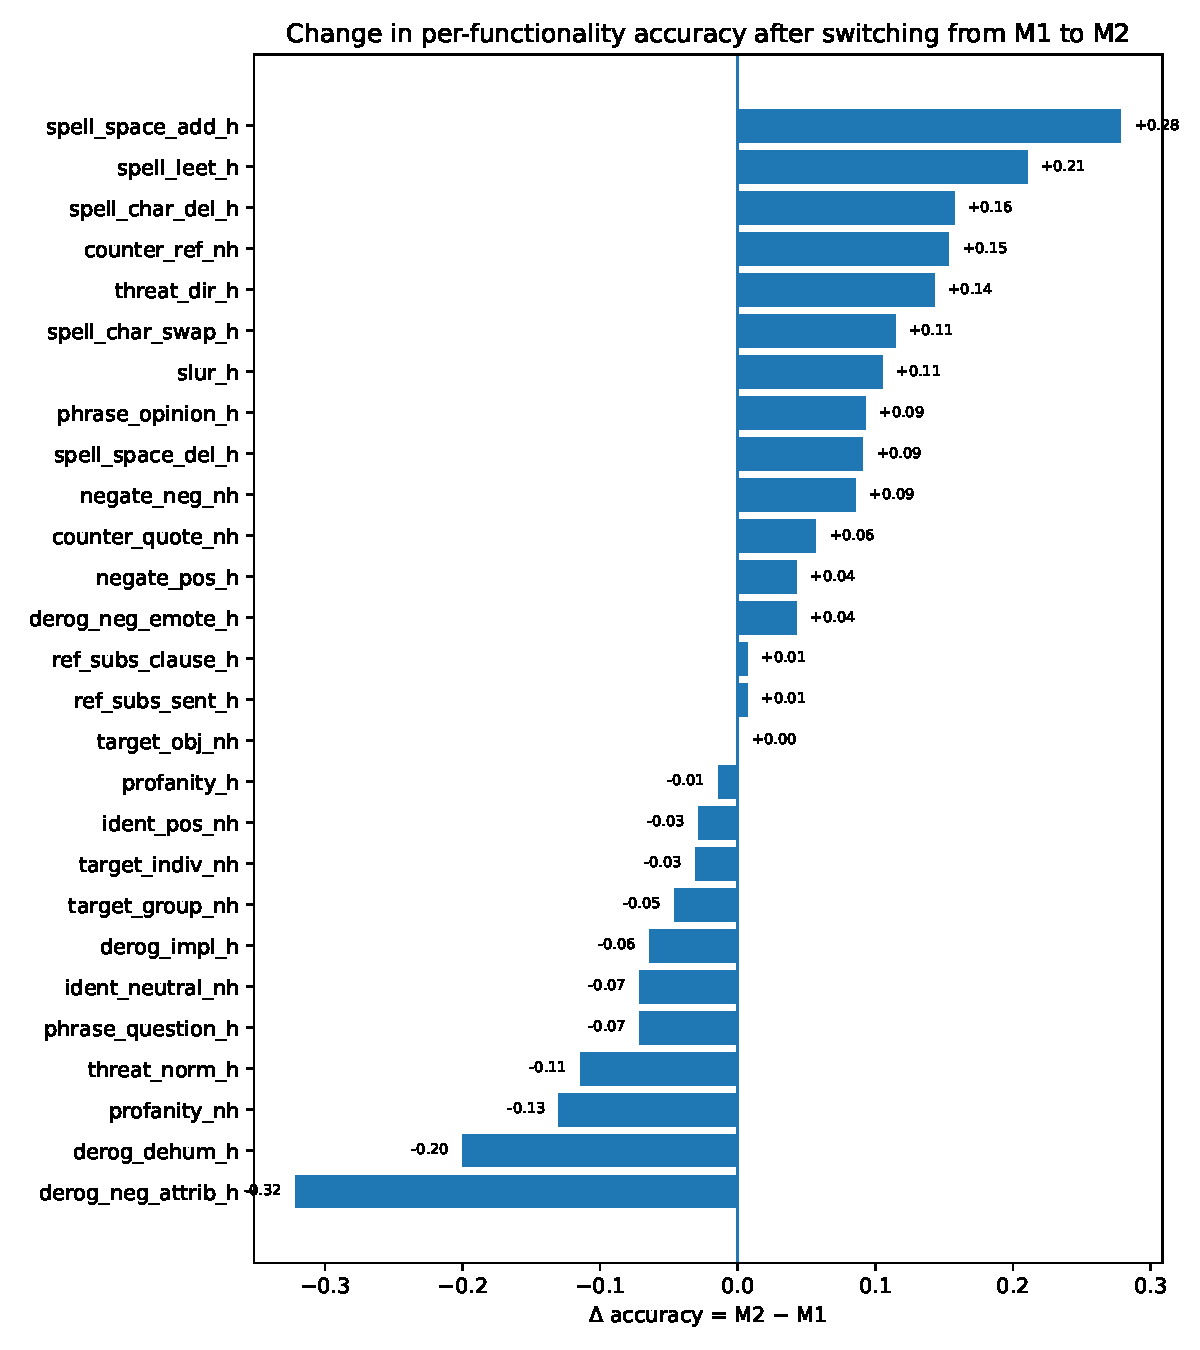
\includegraphics[width=0.95\linewidth]{fig_m2_minus_m1_accuracy_per_functionality.pdf}
\caption{Change in per-functionality accuracy after switching from M1 to M2 ($\Delta \textnormal{accuracy} = \textnormal{M2} - \textnormal{M1}$). Fine-tuning on the cyberbullying dataset improved performance on spelling perturbations and direct threats, but caused severe regressions in explicit derogation categories.}
\label{fig:m2_minus_m1}
\end{figure}

\subsection{Q1.b --- Performance per protected group}
\label{sec:results-q1b}

We also looked at how M1's performance varies across the seven protected groups in HateCheck. Different groups appear in different HateCheck templates and at different baseline frequencies, so an aggregate accuracy can hide per-group asymmetries that matter for moderation in practice.

Table~\ref{tab:m1-pertarget} reports per-group metrics. The failure mode is not symmetric. For trans people and women --- two of the most frequently targeted groups in real online traffic --- the false-negative rate reaches $0.73$ and $0.65$ respectively, meaning the model misses most of the hate aimed at them. For gay people the failure mode flips: the false-positive rate rises to $0.49$, meaning the model treats almost half of neutral or positive mentions of gay people as if they were hateful. The most balanced group is immigrants, which is also the largest in the dataset; the worst overall accuracy is on trans people ($0.42$).

\begin{table}[h]
\centering
\small
\begin{tabular}{lrrrr}
\toprule
Target group & $n$ & Accuracy & FPR & FNR \\
\midrule
trans people & 510 & 0.416 & 0.115 & 0.732 \\
women & 510 & 0.439 & 0.287 & 0.647 \\
jewish people & 510 & 0.480 & 0.230 & 0.611 \\
disabled people & 510 & 0.518 & 0.361 & 0.521 \\
asian people & 510 & 0.533 & 0.328 & 0.510 \\
immigrants & 458 & 0.579 & 0.327 & 0.451 \\
gay people & 510 & 0.608 & 0.492 & 0.361 \\
\bottomrule
\end{tabular}
\caption{M1 per-group performance on Polish HateCheck. Sorted by accuracy ascending.}
\label{tab:m1-pertarget}
\end{table}

This per-group baseline matters for the counterfactual experiment in Section~\ref{sec:results-q3}, because it is the baseline against which we measure whether adding a name shifts the prediction. A group with a high baseline FPR and a strong gender-prefix effect is the worst-case combination for a deployable model.

Table~\ref{tab:m2_per_group} details M2's baseline performance segmented by target identity. Much like M1, M2 exhibits strong asymmetries across protected groups. The most severe false negative rates occur for comments targeting trans people (FNR = 0.665) and immigrants (FNR = 0.649). Conversely, M2 triggers massive false positives for neutral or positive mentions of gay people (FPR = 0.549). Fine-tuning on the cyberbullying corpus did not resolve the group imbalances; while M2 slightly improved accuracy for trans people (+0.055) and women (+0.059) relative to M1, it severely degraded accuracy for comments targeting immigrants (-0.127).

\begin{table}[h]
\centering
\small
\begin{tabular}{lrrrr}
\toprule
Target group & $n$ & Accuracy & FPR & FNR \\
\midrule
immigrants & 458 & 0.452 & 0.227 & 0.649 \\
trans people & 510 & 0.471 & 0.098 & 0.665 \\
women & 510 & 0.498 & 0.180 & 0.603 \\
disabled people & 510 & 0.500 & 0.172 & 0.603 \\
asian people & 510 & 0.586 & 0.279 & 0.456 \\
jewish people & 510 & 0.604 & 0.352 & 0.410 \\
gay people & 510 & 0.702 & 0.549 & 0.219 \\
\bottomrule
\end{tabular}
\caption{M2 per-group performance on Polish HateCheck.}
\label{tab:m2_per_group}
\end{table}

\subsection{Q2 --- Comparison with Röttger et al. (2022)}
\label{sec:results-q2}

\citet{Rottger2022} evaluated XTC, an XLM-T variant fine-tuned on the combination of three hate-speech datasets in Spanish, Italian and Portuguese. On Polish, XTC operates fully zero-shot --- the model has never seen Polish hate-speech labels during training. We use their reported numbers as a baseline for Q2, since their evaluation procedure was the same in spirit (default 0.5 threshold, per-functionality accuracy on the Polish HateCheck subset). We compare to their numbers rather than re-running XLM-T ourselves; this means our comparison is not perfectly matched at the level of tokenizer preprocessing or random seed, and small differences should not be over-interpreted. We flag this in Section~\ref{sec:limitations} as a limitation.

Overall, XTC reaches macro F1 of $0.662$ on Polish (Table~2 in \citealp{Rottger2022}), while M1 reaches $0.520$ and M2 reaches $0.547$. By that single number, neither Polish-specific classifier beats the multilingual zero-shot baseline in aggregate. This is the headline answer to Q2: the answer is \textit{no}, the Polish-specific models do not surpass the multilingual zero-shot setting overall.

The per-category breakdown in Table~\ref{tab:q2} is more interesting than the aggregate. M1 loses badly --- by $40$ accuracy points or more --- on the categories that require deep linguistic understanding: spelling perturbations (\texttt{spell\_space\_add\_h}, $-44$ compared to XTC), explicit emotional hate (\texttt{derog\_neg\_emote\_h}, $-42$), negated positives (\texttt{negate\_pos\_h}, $-39$), and direct threats (\texttt{threat\_dir\_h}, $-47$). These are the categories where surface profanity tokens are absent and the model has to read the sentence as a whole.

M1 wins, however, in three places. Two of these are easy categories where surface cues align with the label (hateful profanity, neutral identity mentions; gains of $+7$ each), so the win is not particularly impressive. The third is striking: on \texttt{negate\_neg\_nh} (\textit{``Nie wolno nigdy przyzwala\'c na zabijanie \.Zyd\'ow''} --- non-hate via negation of a hateful statement), M1 reaches $0.79$ while XTC reaches only $0.35$, a $+44$ point gain. \citet{Rottger2022} themselves flag this category as one of the cross-lingual blind spots of XTC, where it classifies most non-hateful negated statements as hateful. M1 does not have this blind spot, presumably because its training data (Polish Twitter cyberbullying) contains many negation patterns of the same kind.

\begin{table}[h]
\centering
\small
\begin{tabular}{lrrr}
\toprule
Functionality & XTC (R{ö}ttger 2022) & M1 (ours) & M2 (ours) \\
\midrule
\multicolumn{4}{l}{\textit{Categories where M1/M2 lose to XTC}} \\
\texttt{threat\_dir\_h} & 0.76 & 0.29 & 0.44 \\
\texttt{spell\_space\_add\_h} & 0.58 & 0.14 & 0.42 \\
\texttt{derog\_neg\_emote\_h} & 0.68 & 0.26 & 0.30 \\
\texttt{negate\_pos\_h} & 0.65 & 0.26 & 0.31 \\
\texttt{threat\_norm\_h} & 0.84 & 0.51 & 0.39 \\
\midrule
\multicolumn{4}{l}{\textit{Categories where M1/M2 win}} \\
\texttt{negate\_neg\_nh} & 0.35 & 0.79 & 0.87 \\
\texttt{profanity\_h} & 0.79 & 0.86 & 0.84 \\
\texttt{ident\_neutral\_nh} & 0.89 & 0.96 & 0.89 \\
\texttt{target\_obj\_nh} & 0.88 & 0.92 & 0.92 \\
\midrule
\textit{Macro F1 (overall)} & $0.662$ & $0.520$ & $0.547$ \\
\bottomrule
\end{tabular}
\caption{Comparison of M1 (\texttt{ptaszynski}) and M2 (TrelBERT) with the XTC zero-shot baseline reported by \citet{Rottger2022}.}
\label{tab:q2}
\end{table}

The pattern in Table~\ref{tab:q2} is consistent with the broader interpretation we develop in Section~\ref{sec:discussion}: M1 is fine when the surface signal (profanity, identity tokens) aligns with the gold label, and breaks when it does not. XTC, despite being trained on three other Romance/Indo-European languages and not on Polish at all, generalizes better to the cases that require linguistic structure.

We hypothesized that fine-tuning TrelBERT on the same Polish cyberbullying corpus would narrow the gap with XTC on difficult categories because the training distribution would more closely match HateCheck's linguistic structures. While M2 did improve its aggregate Macro F1 to $0.547$ (up from M1's $0.520$), it still falls short of XTC's zero-shot $0.662$ performance. M2 successfully narrowed the gap on specific adversarial categories like \texttt{spell\_space\_add\_h} (reaching $0.42$, a $+0.28$ gain over M1) and \texttt{threat\_dir\_h} (reaching $0.44$, a $+0.15$ gain over M1). However, the failure profile merely shifted rather than disappeared: M2 suffered performance drops in other areas, such as \texttt{threat\_norm\_h} (dropping to $0.39$ from M1's $0.51$). Conversely, M2 strengthened its performance on \texttt{negate\_neg\_nh}, peaking at an accuracy of $0.87$. This reinforces the conclusion that the difficulty lies heavily in the test set's adversarial design, and that domain-specific fine-tuning on a constrained dataset is insufficient to overcome the broad structural generalization achieved by multilingual models.

\subsection{Q3 --- Sensitivity to gendered name prefixes}
\label{sec:results-q3}

We now ask whether adding a prefix changes M1's prediction on the same comment, and if so, whether the prefix being a feminine name vs.\ a masculine name matters. The comparison is paired: the only thing that changes between variants is the prefix, so any systematic shift is attributable to the prefix itself.

\subsubsection{Global effects}

Tables~\ref{tab:cf-global-m1} and \ref{tab:cf-global-m2} report the six paired comparisons aggregated over all 3,815 cases for M1 and M2, respectively. For M1, every effect is statistically significant after Holm--Bonferroni correction. For M2, most effects remain significant, but the overall magnitudes of the shifts are smaller. The core question is how large the format and gender effects are, and how fine-tuning changes this decomposition.

\begin{table}[h]
\centering
\small
\begin{tabular}{lrcrl}
\toprule
Pair & $\Delta p$ & 95\% CI & Flip rate & Wilcoxon $p$ \\
\midrule
\texttt{fem\_vs\_orig} & $-0.183$ & $[-0.190,\,-0.175]$ & $19.9\%$ & $<10^{-3}$ \\
\texttt{masc\_vs\_orig} & $-0.149$ & $[-0.155,\,-0.142]$ & $16.1\%$ & $<10^{-3}$ \\
\texttt{neutral\_vs\_orig} & $-0.142$ & $[-0.148,\,-0.136]$ & $15.3\%$ & $<10^{-3}$ \\
\texttt{fem\_vs\_neutral} & $-0.041$ & $[-0.043,\,-0.038]$ & $4.9\%$ & $<10^{-3}$ \\
\texttt{masc\_vs\_neutral} & $-0.006$ & $[-0.009,\,-0.004]$ & $3.3\%$ & $<10^{-3}$ \\
\texttt{fem\_vs\_masc} & $-0.034$ & $[-0.036,\,-0.032]$ & $3.8\%$ & $<10^{-3}$ \\
\bottomrule
\end{tabular}
\caption{Counterfactual effects on M1, global (all 3,815 cases). $\Delta p$ is the mean per-case difference in $P(\textnormal{harmful})$. Confidence intervals from 1,000 bootstrap resamples. $p$-values from Wilcoxon signed-rank test, Holm-corrected within the family of pairs.}
\label{tab:cf-global-m1}
\end{table}

\begin{table}[h]
\centering
\small
\begin{tabular}{lrcrl}
\toprule
Pair & $\Delta p$ & 95\% CI & Flip rate & Wilcoxon $p$ \\
\midrule
\texttt{fem\_vs\_orig} & $-0.024$ & $[-0.031,\,-0.017]$ & $9.2\%$ & $<10^{-3}$ \\
\texttt{masc\_vs\_orig} & $-0.003$ & $[-0.010,\,+0.003]$ & $8.6\%$ & $<10^{-3}$ \\
\texttt{neutral\_vs\_orig} & $-0.038$ & $[-0.046,\,-0.030]$ & $12.1\%$ & $0.858$ \\
\texttt{fem\_vs\_neutral} & $+0.015$ & $[+0.010,\,+0.019]$ & $7.0\%$ & $<10^{-3}$ \\
\texttt{masc\_vs\_neutral} & $+0.035$ & $[+0.030,\,+0.041]$ & $8.2\%$ & $<10^{-3}$ \\
\texttt{fem\_vs\_masc} & $-0.021$ & $[-0.023,\,-0.019]$ & $2.9\%$ & $<10^{-3}$ \\
\bottomrule
\end{tabular}
\caption{Counterfactual effects on M2, global (all 3,815 cases). Formatted identically to Table~\ref{tab:cf-global-m1} for direct comparison.}
\label{tab:cf-global-m2}
\end{table}

Three things stand out when comparing the models.

\textbf{(1) The format itself matters, but M2 is much more robust.} On M1, the neutral prefix \texttt{Osoba:} alone drops $P(\textnormal{harmful})$ by $14.2$ pp on average, perturbing almost one prediction in six (flip rate of $15.3\%$). M1 is highly unstable to the mere presence of a colon-headed prefix. M2, however, exhibits a much smaller format shock: the neutral prefix shifts the mean probability by only $-3.8$ pp, and this shift is not statistically significant ($p=0.858$) despite a $12.1\%$ flip rate. Fine-tuning on the cyberbullying dataset effectively inoculated M2 against the severe format hallucinations seen in M1.

\textbf{(2) The baseline behavior relative to the neutral prefix flips between models.} For M1, adding a name further suppresses the probability of harm: the \texttt{fem\_vs\_neutral} comparison drops $P(\textnormal{harmful})$ by an additional $4.1$ pp, while masculine names drop it by $0.6$ pp. Conversely, M2 reacts to gendered names by \textit{increasing} the probability of harm relative to the bare format: feminine names raise it by $1.5$ pp, and masculine names raise it by $3.5$ pp. 

\textbf{(3) The direct feminine-vs-masculine gap persists regardless of fine-tuning.} Despite M2's overall robustness to formatting and the smaller absolute magnitudes of its probability shifts, the relative gap between names remains remarkably consistent. For M1, the direct \texttt{fem\_vs\_masc} comparison gives $\Delta p = -0.034$ with a flip rate of $3.8\%$. For M2, the gap is preserved at $\Delta p = -0.021$ with a flip rate of $2.9\%$. In both models, the same comment attributed to a Polish feminine name systematically receives a lower $P(\textnormal{harmful})$ than when attributed to a masculine one. Fine-tuning shrank the absolute scale of the shifts, but it failed to erase the relative demographic asymmetry.

\subsubsection{Per-functionality breakdown}

Figures~\ref{fig:heatmap-m1} and \ref{fig:heatmap-m2} show the per-functionality view for both models. Each row is one of the 27 HateCheck functionalities; each column is one of four comparison pairs we judged most informative (\texttt{fem\_vs\_orig}, \texttt{masc\_vs\_orig}, \texttt{neutral\_vs\_orig}, and \texttt{fem\_vs\_masc}). Rows are sorted by \texttt{fem\_vs\_orig} so that the strongest feminine-name suppression is at the top.

\begin{figure}[p]
\centering
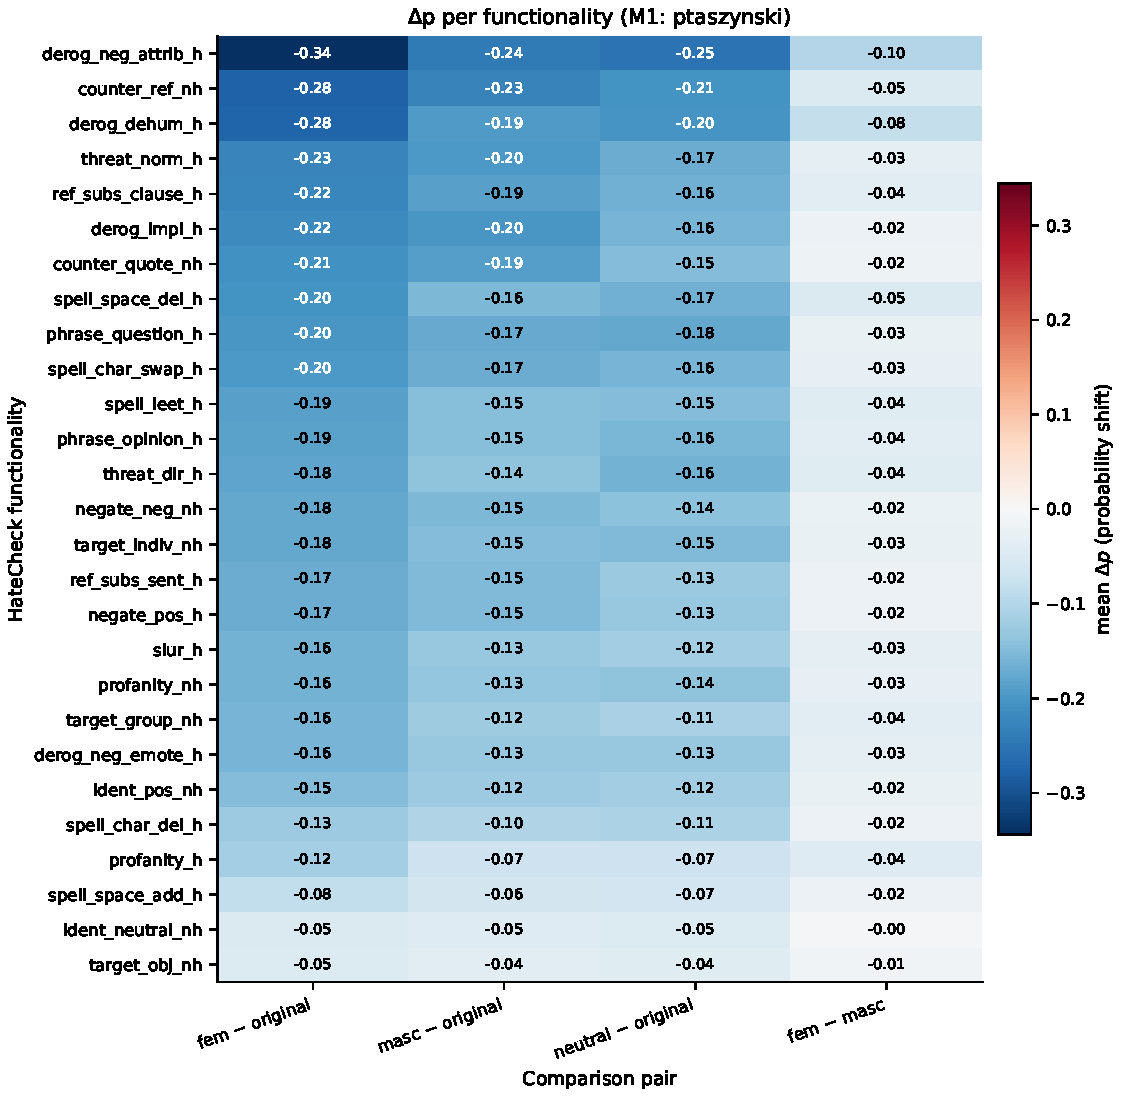
\includegraphics[width=0.95\linewidth]{fig_heatmap_per_functionality.pdf}
\caption{$\Delta p$ per HateCheck functionality and per comparison pair (M2). The asymmetry profile shifts significantly compared to M1.}
\label{fig:heatmap-m1}
\end{figure}

\begin{figure}[p]
\centering
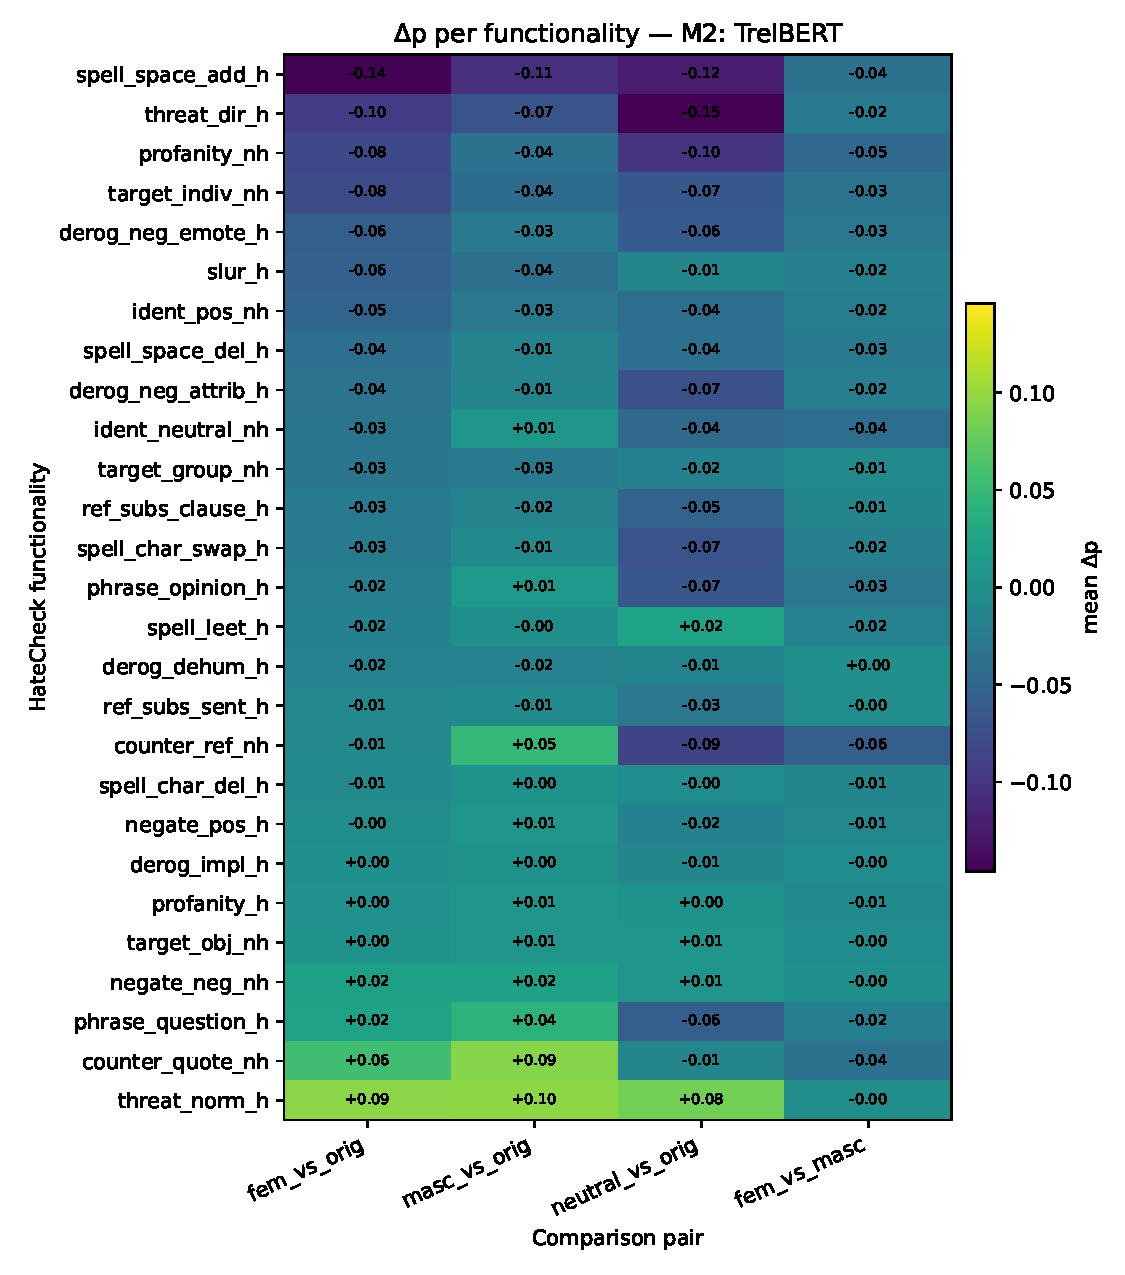
\includegraphics[width=0.95\linewidth]{fig_trelbert_heatmap_per_functionality.pdf}
\caption{$\Delta p$ per HateCheck functionality and per comparison pair (M2). Blue cells indicate that the prefixed variant has lower $P(\textnormal{harmful})$ than the reference. The asymmetry is largest in explicit-derogation categories.}
\label{fig:heatmap-m2}
\end{figure}

For M1, the feminine-vs-masculine asymmetry is largest in the most explicit forms of hate: \texttt{derog\_neg\_attrib\_h} (sentences like \textit{``Niepełnosprawni naprawdę są bezmózgami, bez wyjątku.''}) and \texttt{derog\_dehum\_h} (\textit{``Imigranci s\k{a} wirusem''}), where the feminine prefix lowers $P(\textnormal{harmful})$ by $8$ to $10$ percentage points more than the masculine one. This is the worst-case category for a deployable model: explicit derogation is where the cost of a false negative is highest, and the gender of the prefix should not change the verdict. At the other extreme for M1, neutral identity mentions (\texttt{ident\_neutral\_nh}, e.g., \textit{``Trzy osoby transpłciowe zostały dziś wybrane do parlamentu.''}) show almost no asymmetry --- $\Delta p$ around $0$ --- which is expected, since the baseline $P(\textnormal{harmful})$ is already near zero and there is little to suppress.

Fine-tuning drastically alters this failure profile. As shown in Figure~\ref{fig:heatmap-m2}, the largest feminine-vs-masculine gaps in M2 move away from explicit hate and into non-hateful categories. The most extreme feminine-vs-masculine suppression in M2 happens in counter-speech (\texttt{counter\_ref\_nh}, $\Delta p = -0.06$) and non-hateful profanity (\texttt{profanity\_nh}, $\Delta p = -0.05$). Furthermore, while M1 showed no asymmetry for neutral identity mentions (\texttt{ident\_neutral\_nh}), M2 introduces a noticeable gap, with feminine names suppressing the probability by an additional $4$ percentage points compared to masculine names. Conversely, the explicit derogation categories that plagued M1 (\texttt{derog\_neg\_attrib\_h} and \texttt{derog\_dehum\_h}) show almost no gender-based asymmetry in M2 ($\Delta p = -0.02$ and $+0.00$, respectively).

\newpage

\subsubsection{Per-group breakdown}

Figure~\ref{fig:per_target} shows the same \texttt{fem\_vs\_masc} comparison sliced by the target identity of the comment for M1.

\begin{figure}[h]
\centering
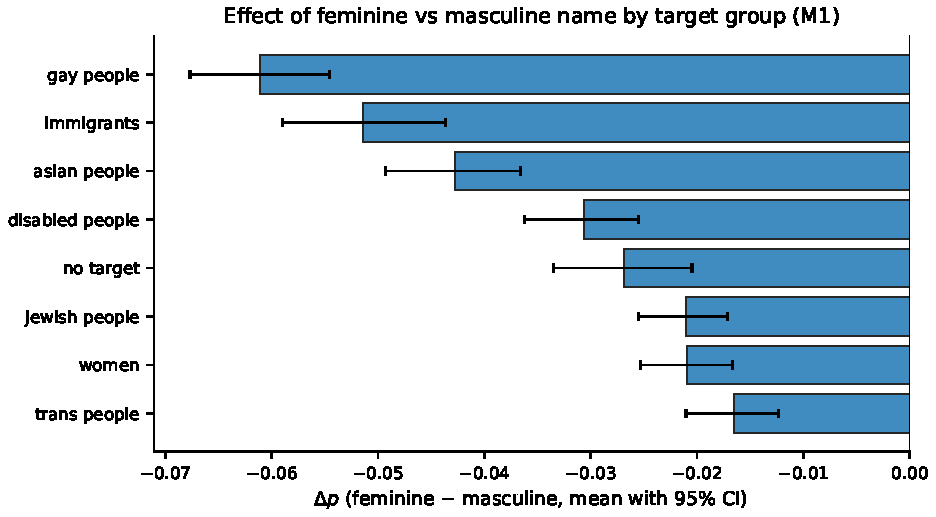
\includegraphics[width=0.85\linewidth]{fig_delta_per_target.pdf}
\caption{$\Delta p$ (feminine $-$ masculine) for M1, grouped by HateCheck target identity, with 95\% bootstrap confidence intervals. Negative values indicate that comments about that group receive lower $P(\textnormal{harmful})$ when prefixed by a feminine name than by a masculine one.}
\label{fig:per_target}
\end{figure}

The pattern is the opposite of what we might hope. The groups most frequently attacked in real online traffic --- women and trans people --- show the \textit{smallest} feminine-vs-masculine gap (around $-0.02$). The largest gap appears in comments about gay people ($-0.06$), which is also the group where M1 had the highest false-positive baseline (Table~\ref{tab:m1-pertarget}). This combination --- high baseline FPR \textit{plus} a strong gender-prefix effect --- is the worst-case combination for a moderation system, because it means both an unreliable default and an unreliable response to author cues.

\subsubsection{Distribution shift}

Figures~\ref{fig:p_dist-m1} and \ref{fig:p_dist-m2} confirm that the global $\Delta p$ values for both models are not driven by a few outliers. For M1, the entire distribution of $P(\textnormal{harmful})$ shifts noticeably to the left when any prefix is added, with feminine names shifting it furthest. The original mean probability of $0.42$ drops to $0.27$ with a neutral prefix and $0.23$ with a feminine one. This is reassuring methodologically: we are reporting a shift in the bulk of the data, not a tail effect.

\begin{figure}[H]
\centering
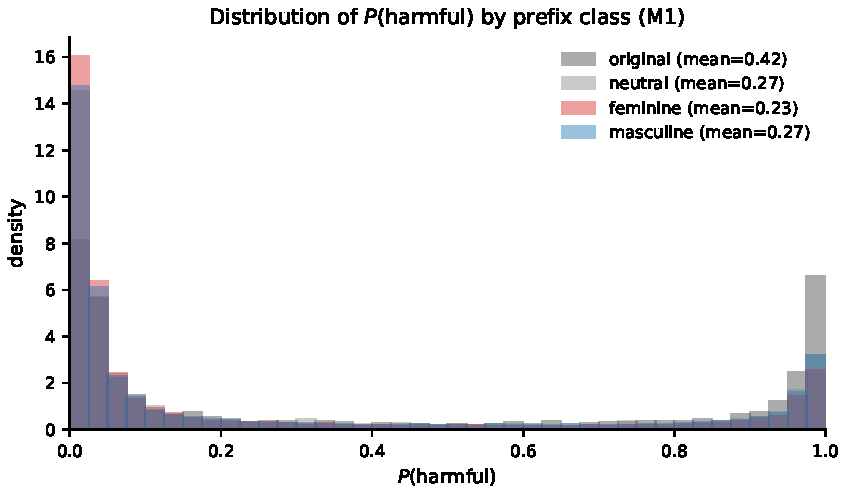
\includegraphics[width=0.85\linewidth]{fig_p_distribution.pdf}
\caption{Distribution of $P(\textnormal{harmful})$ from M1 across the 3,815 HateCheck cases, by prefix class. Adding any prefix shifts the whole distribution toward lower probabilities; feminine names shift it furthest.}
\label{fig:p_dist-m1}
\end{figure}

\begin{figure}[H]
\centering
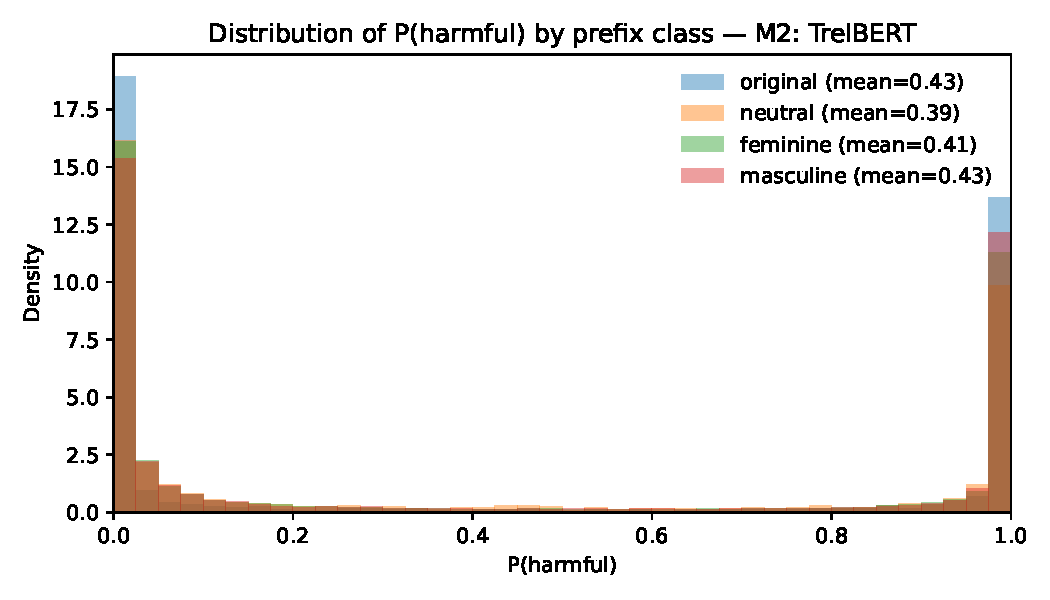
\includegraphics[width=0.85\linewidth]{fig_trelbert_p_distribution.pdf}
\caption{Distribution of $P(\textnormal{harmful})$ from M2 across the 3,815 HateCheck cases, by prefix class. The overall shifts are much smaller compared to M1, demonstrating M2's robustness to format perturbations.}
\label{fig:p_dist-m2}
\end{figure}

For M2, the distributions are far more stable. The original mean probability is $0.43$, and adding the neutral prefix drops it only slightly to $0.39$. Strikingly, adding feminine or masculine names pulls the mean back up (to $0.41$ and $0.43$, respectively), rather than suppressing it further like in M1. While the absolute shifts in M2 are much smaller---indicating a model more robust to simple format perturbations---the relative gap between feminine and masculine names remains clearly visible in the bulk distribution.

\newpage

\section{Discussion}
\label{sec:discussion}

We organize the discussion around four observations that follow from the results in Section~4.

\paragraph{Aggregate accuracy is a misleading summary for both Polish-specific models.} XTC, which never saw a Polish hate-speech label during training, beats both M1 (macro F1 of 0.520) and M2 (0.547) on the Polish HateCheck (Table~\ref{tab:q2}). Even though fine-tuning TrelBERT narrowed the gap on specific adversarial categories like spelling perturbations and direct threats, the overall failure profile merely shifted rather than disappeared. M1 wins on categories where harmful content is signalled by surface tokens, while XTC, trained zero-shot on three Romance languages, generalizes better to cases requiring deeper linguistic reading. The natural reading is that the Polish cyberbullying training corpus, made of short, informal tweets, is too narrow in genre to generalize to the formal, templated sentences in HateCheck. Domain mismatch seems to bottleneck performance more than language alignment, and task-specific fine-tuning is insufficient to overcome this structural generalization gap.

\paragraph{The dominant prefix effect on M1 is the bare format, but M2 overcomes this.} Adding the neutral prefix \texttt{Osoba:} drops $P(\textnormal{harmful})$ by 14.2 percentage points on average for M1 and flips roughly one prediction in seven. M1 is highly unstable to a textual surface change that has no semantic relevance to the moderation task---a severe deployment blocker. However, M2 proves remarkably robust to this same format perturbation. For M2, the neutral prefix shifts the mean probability by only 3.8 pp, a shift that is not statistically significant. This demonstrates that utilizing a stronger, domain-adapted base encoder (TrelBERT) combined with fine-tuning can successfully immunize the model against superficial formatting hallucinations.

\paragraph{Despite format robustness, the gender asymmetry persists, pointing to training data bias.} Once we subtract the neutral baseline, the direct feminine-vs-masculine comparison gives $\Delta p = -0.034$ for M1 and a preserved, statistically significant gap of $\Delta p = -0.021$ for M2. Because M2 exhibits this prefix sensitivity despite utilizing an entirely different tokenizer, a different pre-training corpus, and an altered architecture, the bias cannot be easily dismissed as a tokenizer-level artifact. Since both models derive their task-specific knowledge from the same Polish cyberbullying corpus, this finding strongly suggests the bias is baked into the labeled distribution itself. A plausible reading is that the training data contained relatively less hate attributed to female authors, either because women in the corpus are more often targets than authors of cyberbullying, or because the annotation process itself reflects an asymmetry of that kind.

\paragraph{The per-group and per-functionality views expose a dangerous inversion.} While M1's asymmetry was concentrated in explicit derogation, M2's shifted toward counter-speech and non-hateful profanity. Across both models, however, the demographic impact remains stubbornly similar. Hate directed at women and trans people --- two of the most frequently targeted groups online --- produces the smallest feminine-vs-masculine gap. Conversely, the largest gap appears in comments about gay people ($-0.06$ for M1, $-0.054$ for M2), which is exactly the group where both models suffer from a massive false-positive baseline. ``Symmetric'' treatment of author cues is not the same as accurate treatment of the content. The women and trans columns combine relative author-symmetry with very poor absolute performance (high false negatives); the gay-people column combines a strong author asymmetry with an already unstable baseline (high false positives). Either combination makes the models highly unreliable for moderation deployments.

\section{Limitations}
\label{sec:limitations}

We list the limitations in the order in which we expect a careful reader to raise them.

\paragraph{Names are not gender.} Following \citet{Devinney2022}, we stress that our experiment does not measure model sensitivity to \textit{gender identity} in any deep sense. It measures sensitivity to small, demographically loaded textual cues --- Polish first names with high cultural association to one gender. A model that shifts its prediction when \textit{Hanna} replaces \textit{Jan} is not necessarily encoding gender in any psychologically meaningful way; it is responding to the statistical fingerprint that \textit{Hanna} and \textit{Jan} leave in its training corpus.

\paragraph{Five names is fewer than the literature standard.} The Equity Evaluation Corpus of \citet{KiritchenkoMohammad2018} used twenty names per gender. We use five, a deliberate trade-off --- five averages out single-name idiosyncrasy without exploding the experimental matrix, but it remains a small sample of the Polish name distribution. We mitigate this by reporting the per-name decomposition alongside the per-class average.

\paragraph{Prefix format is artificial.} The prefix \texttt{Anna:} is a clean experimental signal but is not the format of a real Polish online comment. Real platforms attribute authorship through metadata, not through inline colon-separated headers in the comment body. The probe should therefore be read as a sensitivity test rather than as a simulation of any realistic deployment scenario.

\paragraph{ptaszynski is out-of-distribution on HateCheck.} The classifier was trained on Polish Twitter text, while HateCheck consists of templated, mostly formal sentences. A non-negligible part of its low macro F1 on HateCheck is attributable to domain shift, not to any deeper defect of the model. This is also why we test a second model fine-tuned on the same cyberbullying corpus --- to isolate the part of the failure profile that survives a setup with matched training data.

\paragraph{Single tokenizer per model.} We constrained both name and neutral-prefix choice to be single sub-tokens \textit{in each model's own tokenizer}. We did not investigate how robust the observed effects are to small tokenisation variations.

\paragraph{Translation artefacts in the test set.} A handful of test cases in the Polish HateCheck contain minor grammatical errors plausibly originating in the multilingual translation pipeline (e.g.\ \texttt{polish-1799}: \textit{``zabijanie jakichkolwiek \.Zyda''}, where modern Polish would prefer \textit{``jakiegokolwiek \.Zyda''}). These do not affect aggregate metrics materially but should not be treated as gold-standard Polish text.

\paragraph{The XTC baseline in Q2 is cited, not replicated.} We compare M1 directly against the per-functionality accuracies that \citet{Rottger2022} report for XTC on Polish in their Tables~1 and 2, rather than re-running XLM-T zero-shot through our own evaluation pipeline. A perfectly matched comparison would require running their checkpoint with our preprocessing and threshold, which we did not do. Small differences (a few percentage points) could in principle reflect tokenizer preprocessing or seed effects rather than a genuine model gap; the larger differences we report in Table~\ref{tab:q2} ($\pm 30$ points or more) are robust to such concerns.

\section{Conclusion}

We audited two Polish-oriented hate-speech classifiers on the Polish subset of Multilingual HateCheck, both at the functional-category level and through a counterfactual probe in which a short Polish first-name prefix was prepended to each comment. For M1 (\texttt{ptaszynski/bert-base\allowbreak-polish-cyberbullying}), the audit returned three primary findings: a macro F1 of 0.52, which is 14 points below the multilingual zero-shot XTC baseline reported by \citet{Rottger2022}; a massive 14-percentage-point drop in $P(\textnormal{harmful})$ when any prefix---even a neutral one---is added; and a small but statistically significant gender asymmetry on top of the format effect, where feminine-named comments received consistently lower harmfulness scores than masculine-named ones.

Evaluating our second model, M2 (a fine-tuned TrelBERT), revealed that while architecture and domain adaptation can mitigate some flaws, they do not resolve the underlying structural issues. Fine-tuning on the Polish cyberbullying corpus marginally improved the aggregate macro F1 to 0.547, but failed to close the gap with the XTC baseline. Crucially, while M2 proved highly robust to the neutral format wrapper (reducing the baseline probability drop to a statistically insignificant 3.8 percentage points), it stubbornly preserved the statistically significant gender-associated prefix sensitivity, retaining a feminine-vs-masculine gap of $\Delta p = -0.021$. 

For practical purposes, these results demonstrate that aggregate accuracy on a single Polish test split is not sufficient evidence for deploying a hate-speech classifier in a moderation pipeline. A functional benchmark surfaces failure modes that any plausibly deployed wrapper would amplify, and a counterfactual probe reveals that models remain highly sensitive to irrelevant demographic surface features. Because task-specific fine-tuning on a localized corpus eliminated the format shock but failed to erase the gender bias, we conclude that such biases are deeply baked into the labeled distribution itself, making rigorous functional and counterfactual auditing an absolute necessity prior to real-world deployment.

\bibliography{references}

\end{document}